\subsection{Leitungskonstanten direkt}
Die gemessenen Werte für $R,C,L$ für die beiden Kabel stehen in den Tabellen \ref{tab:RLC50Werte} und \ref{tab:RLC75Werte}. Die Werte für $G$ werden berechnet, indem
eine verzerrungsfreie Übertragung angenommen wird, d.h. der Phasenbelag $k$ aus \eqref{eq:LosungTelegraph} muss verschwinden. Daraus ergibt sich die Bedingung
\begin{align}
	G = -\frac{RL}{C} \quad.
\end{align}
Mit Hilfe von \eqref{eq:RLCTheorie} können folgende theoretische Vergleichswerte ausgerechnet werden
\begin{align}
	R &= \SI{122.6}{\micro\ohm\per\meter}
 \notag \\
	C &= \SI{105.4}{\pico\farad\per\meter}
 \notag \\
	L &= \SI{237.4}{\nano\farad\per\meter}
 \notag \\
	G &= \SI{54.4}{\nano\siemens\per\meter}
 \quad,
\end{align}
die zusammen mit den Messwerten in den Abbildungen \ref{fig:PlotR} - \ref{fig:PlotG} abgebildet sind.
\begin{table}
    \centering
    \caption{Beim Kurzschließen des $50\Omega$-Kables gemessene Werte für $R_{50},C_{50},L_{50}$ und daruas berechnete Werte für $G_{50}$ bei den jeweils eingestellten Frequenzen $f$}
    \label{tab:RLC50Werte}
    \sisetup{parse-numbers=false}
    \begin{tabular}{
	S[table-format=3.1]
	S[table-format=1.4]
	S[table-format=3.1]
	S[table-format=1.2]
	S[table-format=1.1]
	}
	\toprule
	{$f_{50} \ \mathrm{in} \ \si{\kilo\hertz}$}		& {$R_{50} \ \mathrm{in} \ \si{\ohm}$}		& 
	{$C_{50} \ \mathrm{in} \ \si{\pico\farad}$}		& {$L_{50} \ \mathrm{in} \ \si{\micro\henry}$}		& 
	{$G_{50} \ \mathrm{in} \ \si{\milli\siemens}$}		\\ 
	\midrule
    100.0 & 0.6402 & 987.4 & 3.12 & 0.2 \\
20.0  & 0.5572 & 986.6 & 3.18 & 0.2 \\
18.0  & 0.5556 & 986.6 & 3.18 & 0.2 \\
16.0  & 0.5546 & 986.6 & 3.18 & 0.2 \\
14.0  & 0.5537 & 986.5 & 3.18 & 0.2 \\
12.0  & 0.5530 & 986.5 & 3.18 & 0.2 \\
10.0  & 0.5523 & 986.5 & 3.18 & 0.2 \\
8.0   & 0.5518 & 986.5 & 3.19 & 0.2 \\
6.0   & 0.5513 & 986.5 & 3.19 & 0.2 \\
4.0   & 0.5510 & 986.5 & 3.19 & 0.2 \\
3.0   & 0.5508 & 986.5 & 3.19 & 0.2 \\
2.0   & 0.5506 & 986.5 & 3.18 & 0.2 \\
1.0   & 0.5506 & 986.7 & 3.20 & 0.2 \\
0.8   & 0.5506 & 986.7 & 3.10 & 0.2 \\
0.6   & 0.5505 & 986.7 & 3.10 & 0.2 \\
0.6   & 0.5504 & 986.7 & 3.00 & 0.2 \\
0.2   & 0.5505 & 986.7 & 2.20 & 0.2 \\

    \bottomrule
    \end{tabular}
    \end{table}

\begin{table}
    \centering
    \caption{Beim Kurzschließen des $75\Omega$-Kables gemessene Werte für $R_{75},C_{75},L_{75}$ und daraus berechnete Werte für $G_{75}$ bei den jeweils eingestellten Frequenzen $f$}
    \label{tab:RLC75Werte}
    \sisetup{parse-numbers=false}
    \begin{tabular}{
	S[table-format=3.0]
	S[table-format=1.2]
	S[table-format=3.1]
	S[table-format=1.2]
	S[table-format=1.1]
	}
	\toprule
	{$f_{75} \ \mathrm{in} \ \si{\kilo\hertz}$}		& {$R_{75} \ \mathrm{in} \ \si{\ohm}$}		& 
	{$C_{75} \ \mathrm{in} \ \si{\pico\farad}$}		& {$L_{75} \ \mathrm{in} \ \si{\micro\henry}$}		& 
	{$G_{75} \ \mathrm{in} \ \si{\milli\siemens}$}		\\ 
	\midrule
    100 & 6.90 & 672.5 & 4.28 & 1.1 \\
20  & 6.40 & 671.8 & 5.30 & 0.8 \\
18  & 6.35 & 671.8 & 5.40 & 0.8 \\
16  & 6.30 & 671.7 & 5.51 & 0.8 \\
14  & 6.24 & 671.7 & 5.63 & 0.7 \\
12  & 6.23 & 671.7 & 5.78 & 0.7 \\
10  & 6.11 & 671.7 & 5.91 & 0.7 \\
8   & 6.06 & 671.7 & 6.06 & 0.7 \\

    \bottomrule
    \end{tabular}
    \end{table}

\begin{figure}[h]
	\centering
	\begin{subfigure}{0.496\textwidth}
		\centering
		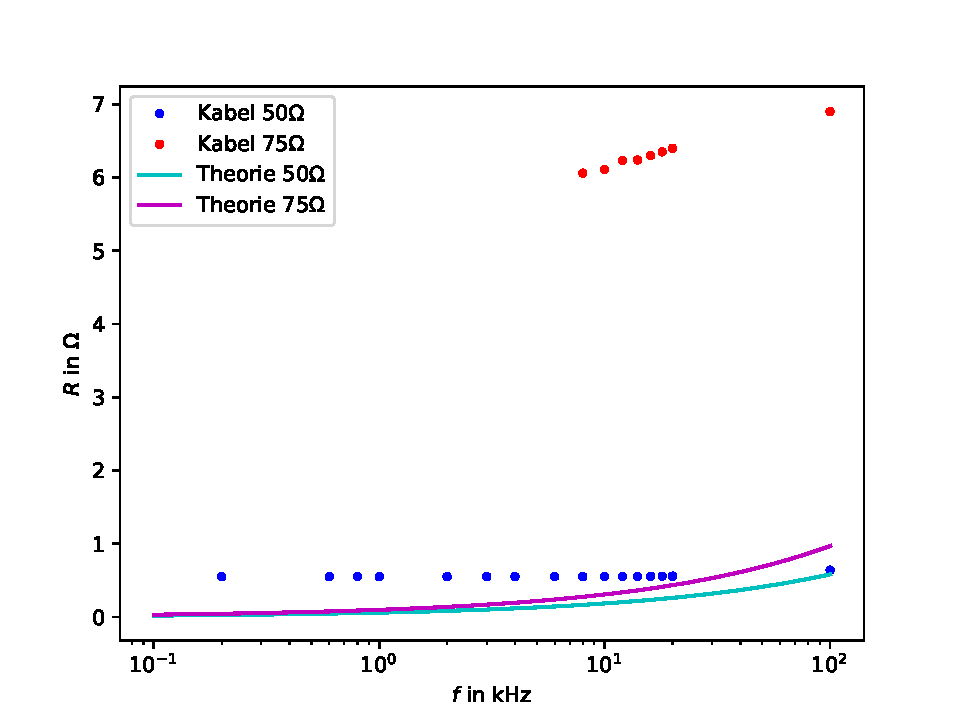
\includegraphics[width=\textwidth]{RLC_DirekteMessung/build/PlotR.pdf}
		\subcaption{Werte für $R$}
		\label{fig:PlotR}
	\end{subfigure}
	\begin{subfigure}{0.496\textwidth}
		\centering
		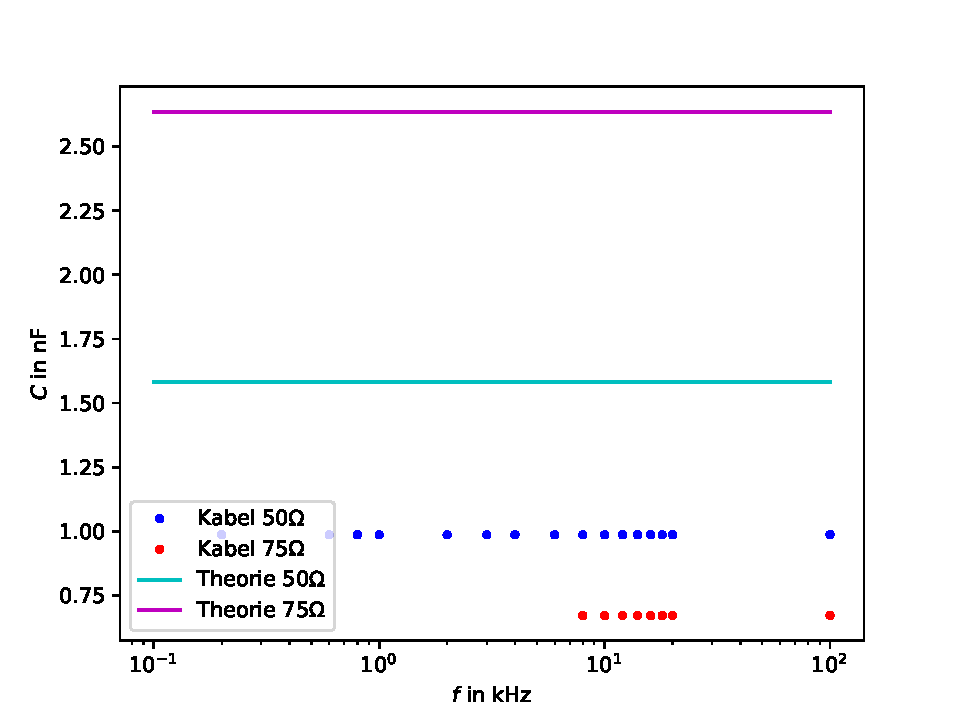
\includegraphics[width=\textwidth]{RLC_DirekteMessung/build/PlotC.pdf}
		\subcaption{Werte für $C$}
		\label{fig:PlotC}
	\end{subfigure}
	\begin{subfigure}{0.496\textwidth}
		\centering
		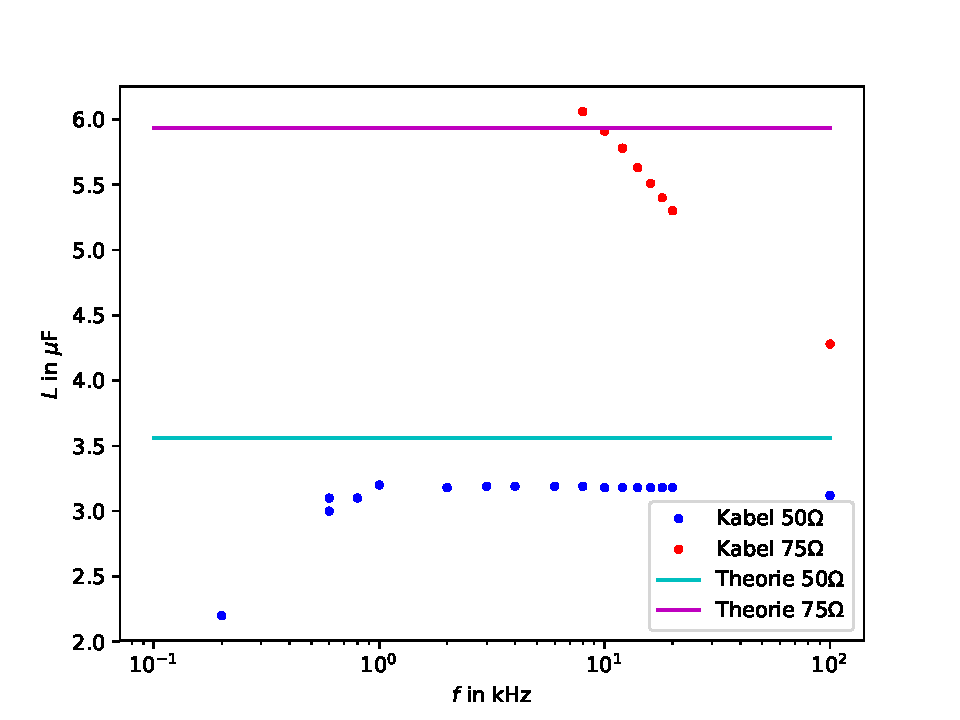
\includegraphics[width=\textwidth]{RLC_DirekteMessung/build/PlotL.pdf}
		\caption{Werte für $L$}
		\label{fig:PlotL}
	\end{subfigure}
	\begin{subfigure}{0.496\textwidth}
		\centering
		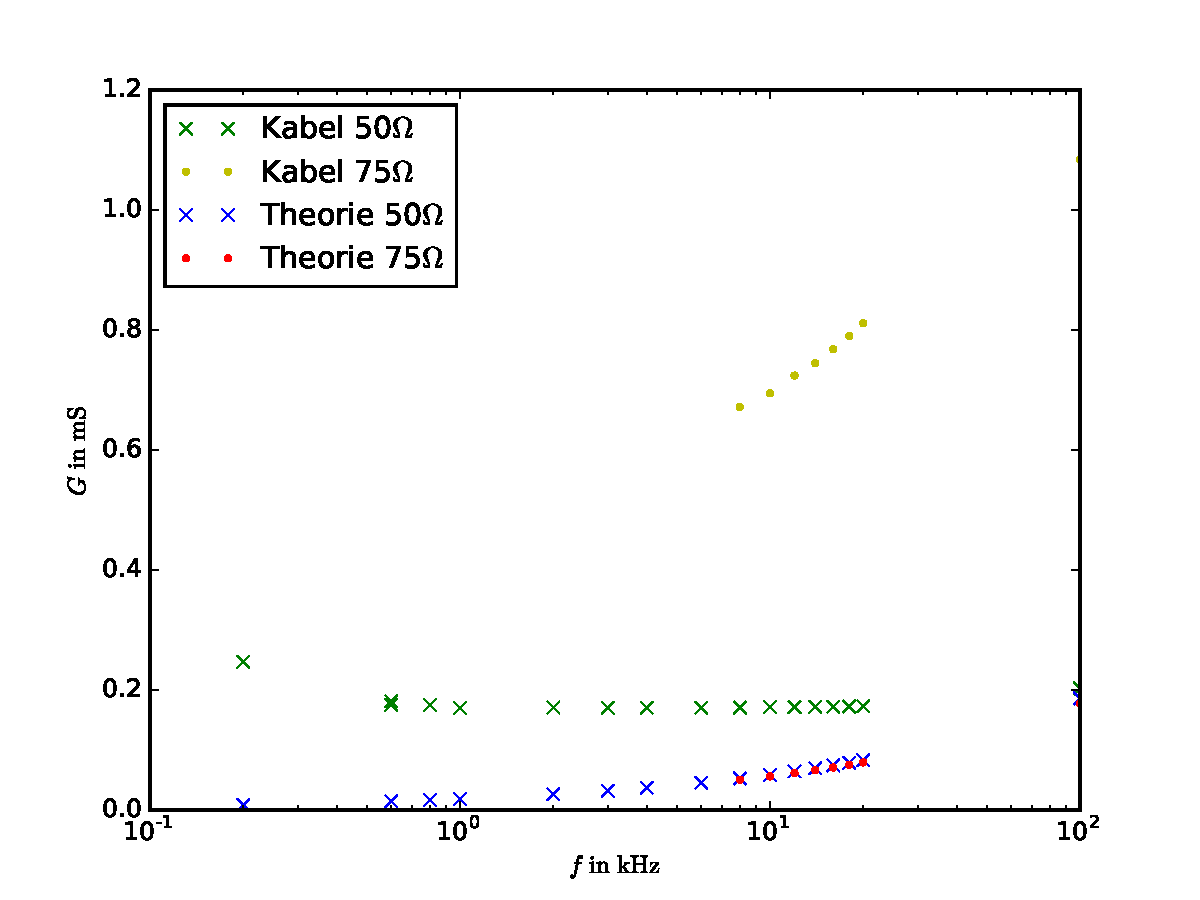
\includegraphics[width=\textwidth]{RLC_DirekteMessung/build/PlotG.pdf}
		\caption{Werte für $G$}
		\label{fig:PlotG}
	\end{subfigure}
	\caption[Werte bei der direkten Messung]{Gemessene Werte für $R,C,L$ bei der direkten Messung, sowie Theoriewerte und berechnete Werte für $G$}
	\label{fig:PlotRLCG}
\end{figure}\clearpage
\subsection{Leitungskonstanten durch Reflexion}
Offenes Ende: Form müsste RC-Parallelschaltung entsprechen. Rechne dafür die Laplace-Trafo aus. Fitte die ausgerechnete Funktion an die Werte. \\
Geschlossenes Ende: Form müsste LR-Reihenschaltung entsprechen. Rechne dafür die Laplace-Trafo aus. Fitte die ausgerechnete Funktion an die Werte.
\subsection{Dämpfungskonstante}
Zur Bestimmung der Dämpfungskonstante wird mit dem Oszilloskop für ein langes und ein kurzes Kabel eine FFT eines Rechteckpulses durchgeführt. Die hier entstandenen Bilder sind in Abbildung \ref{fig:FFT} zu sehen. Die Position und Höhe der Peaks wird aus dem Datensatz extrahiert und sind in Tabelle \ref{tab:DaempfungWerteB} zu sehen. \\
\begin{figure}[h]
	\centering
	\begin{subfigure}{0.495\textwidth}
		\centering
		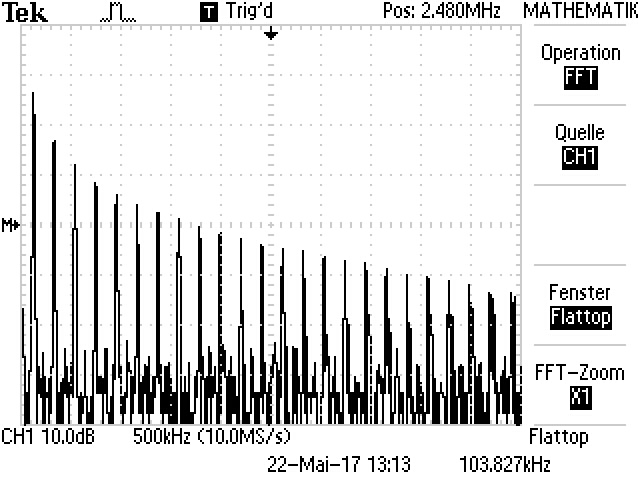
\includegraphics[width=0.9\textwidth]{Oszilloskop/DaempfungLang/F0042TEK.JPG}
		\subcaption{Langes Kabel}
		\label{fig:FFTLang}
	\end{subfigure}
	\begin{subfigure}{0.495\textwidth}
		\centering
		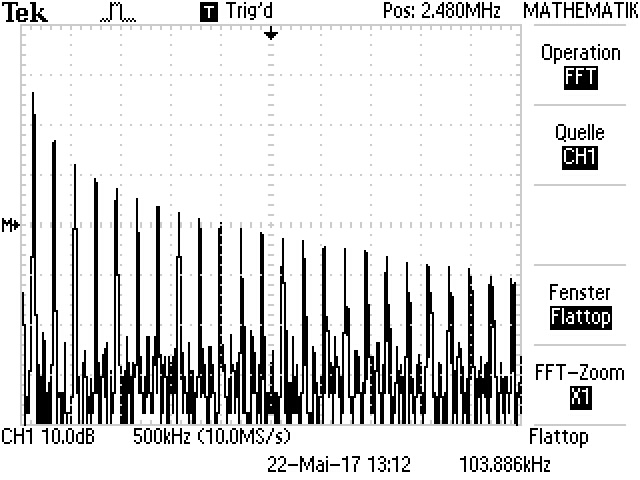
\includegraphics[width=0.9\textwidth]{Oszilloskop/DaempfungKurz/F0041TEK.JPG}
		\subcaption{Kurzes Kabel}
		\label{fig:FFTKurz}
	\end{subfigure}
	\caption{Oszilloskop-Bilder der FFT}
	\label{fig:FFT}
\end{figure}
Da ein ungerades Rechtecksignal betrachtet wird, sind die $\omega_n$ ungerade Vielfache der Grundfrequenz $\omega_0$. Es wird die Vermutung aufgestellt, dass das Oszilloskop die Fouriertransformierte dabei mit
\begin{align}\label{eq:Vermutung}
	P = \ln\left(\frac{U(\omega)}{U_0}\right)
\end{align}
normiert. Die Fourierkoeffizienten und die Fouriertransformierte eines ungeraden Rechtecksignals sind
\begin{align*}
	A_n &=\frac{4U_0}{\pi(2n+1)} = \frac{A_0}{2n+1} \quad, \\
	U(\omega) &= \sum_{n=0}^{\infty}A_n\delta(\omega-\omega_0(2n+1)) \quad.
\end{align*}
Die Amplituden, die das Oszilloskop mit der FFT darstellt können demnach auch durch die Fourierkoeffizienten ausgedrückt werden:
\begin{align}\label{eq:P}
	P_n = \ln\left(\frac{A_n}{A_0}\right) &= \ln\left(\frac{\omega_0}{\omega_n}\right)\notag \\
	&= \ln\left(\frac{\omega_0}{\omega_n}\right)\si{\neper}\notag \quad\footnotemark \\
	&= 20\log_{10}\left(\frac{\omega_0}{\omega_n}\right)\si{\deci\bel} \quad.
\end{align}
Die Grundfrequenz ist dabei
\begin{align*}
	\omega_0 = \frac{\omega(A_n)}{2n+1} = \input{Daempfung/build/omega0} \quad.
\end{align*}
Abbildung \ref{eq:DaempfungB} zeigt diese Amplituden zusammen mit den aus den Messwerten und bestätigt die Vermutung \eqref{eq:Vermutung}, wenn bedacht wird, dass auch beim kurzen Kabel Verluste z.B. an den Verbindungsstücken auftauchen. \footnotetext{\si{\neper} ist eine Einheit, die das Verhältnis von zwei Werten angibt. Sie kann hier einfach hinzugefügt werden, da \SI{1}{\neper} = 1.}
\begin{figure}[h]
	\centering
	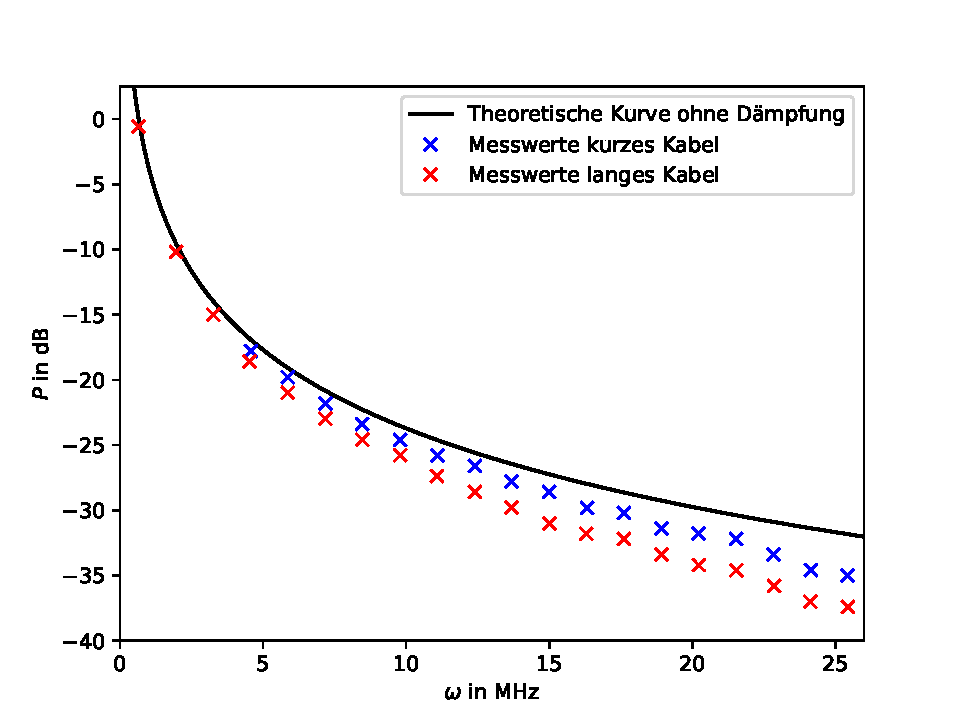
\includegraphics[width=0.8\textwidth]{Daempfung/build/PlotB.pdf}
	\caption{Aus dem Oszilloskop-Datensatz extrahierte Werte der Peaks mit der theoretischen Kurve aus \eqref{eq:P}}
	\label{fig:PlotDaempfungB}
\end{figure} \\
Die Dämpfungskonstante kann nun wie folgt berechnet werden
\begin{align}\label{eq:DaempfungB}
	P_{n,\text{Lang}}-P_{n,\text{Kurz}} &= \ln\left(\frac{U_{n,\text{Lang}}(\omega)}{U_0}\right) - \ln\left(\frac{U_{n,\text{Kurz}}(\omega)}{U_0}\right)\notag \\
	&= \ln\left(\frac{U_{n,\text{Lang}}(\omega)}{U_0}\right) - \ln\left(\frac{U_{n,\text{Kurz}}(\omega)}{U_0}\right)\si{\neper}\notag \\
	&= 20\cdot\log_{10}\left(\frac{U_{n,\text{Lang}}(\omega)}{U_{n,\text{Kurz}}(\omega)}\right)\si{\deci\bel}\notag \\
	&= 20\cdot\log_{10}\left(\exp(-\alpha L)\right)\si{\deci\bel}\notag \\
	&= -20\cdot\alpha\cdot L\cdot\log_{10}e\ \si{\deci\bel}\notag \\
	\Leftrightarrow\quad \alpha &= \frac{P_\text{Lang}-P_\text{Kurz}}{20\cdot L\cdot\log_{10}e\ \si{\deci\bel}} \quad.
\end{align}
Die  Werte für die Dämpfungskonstante sind in Tabelle \ref{tab:DaempfungWerteB} abgebildet. Die Mittelung ergibt
\begin{align}
	\alpha = \SI{3.64+-0.42}{\per\kilo\meter}
 \quad.
\end{align}
\begin{table}
    \centering
    \caption{Frequenz $\omega$ und Betrag der Amplitude $P$ der Peaks in der FFT für das kurze und das lange Kabel, sowie mit \eqref{eq:DaempfungB} berechnete Dämpfung}
    \label{tab:DaempfungWerteB}
    \sisetup{parse-numbers=false}
    \begin{tabular}{
	S[table-format=2.3]
	S[table-format=2.2]
	S[table-format=2.3]
	S[table-format=2.2]
	S[table-format=2.2]
	}
	\toprule
	{$\omega_\text{Kurz} \ \mathrm{in} \ \si{\mega\hertz}$}		& {$|P_\text{Kurz}| \ \mathrm{in} \ \si{\deci\bel}$}		& 
	{$\omega_\text{Lang} \ \mathrm{in} \ \si{\mega\hertz}$}		& {$|P_\text{Lang}| \ \mathrm{in} \ \si{\deci\bel}$}		& 
	{$\alpha \ \mathrm{in} \ \si{\per\kilo\meter}$}		\\ 
	\midrule
    0.644  & 0.59  & 0.644  & 0.59  & -0.00 \\
1.963  & 10.19 & 1.963  & 10.19 & -0.00 \\
3.252  & 14.99 & 3.252  & 14.99 & -0.00 \\
4.571  & 17.79 & 4.541  & 18.59 & 1.84  \\
5.860  & 19.79 & 5.860  & 20.99 & 2.76  \\
7.179  & 21.79 & 7.179  & 22.99 & 2.76  \\
8.468  & 23.39 & 8.468  & 24.59 & 2.76  \\
9.787  & 24.59 & 9.787  & 25.79 & 2.76  \\
11.106 & 25.79 & 11.075 & 27.39 & 3.68  \\
12.395 & 26.59 & 12.395 & 28.59 & 4.61  \\
13.683 & 27.79 & 13.683 & 29.79 & 4.61  \\
15.002 & 28.59 & 15.002 & 30.99 & 5.53  \\
16.322 & 29.79 & 16.291 & 31.79 & 4.61  \\
17.610 & 30.19 & 17.610 & 32.19 & 4.61  \\
18.929 & 31.39 & 18.929 & 33.39 & 4.61  \\
20.218 & 31.79 & 20.218 & 34.19 & 5.53  \\
21.537 & 32.19 & 21.537 & 34.59 & 5.53  \\
22.826 & 33.39 & 22.856 & 35.79 & 5.53  \\
24.145 & 34.59 & 24.114 & 36.99 & 5.53  \\
25.433 & 34.99 & 25.433 & 37.39 & 5.53  \\

    \bottomrule
    \end{tabular}
    \end{table}


\subsection{Abschlusswiderstände}
Finde richtige Kurve in \ref{fig:Zeitkonstanten}. Dann vorgehen wie im 2. Unterkapitel: Fitte e-Funktion mit $\exp(-t/T)$ an den Anstieg bzw. Abfall. Daraus bekommt man die Werte von $C,L,R$.
\subsection{Mehrfachreflexion}
Lese Spannungsdifferenzen ab. Das entspricht dann immer dem jeweiligen Term aus \eqref{eq:Un}. Mit einem Impulsfahrplan überlegt man sich dann wie die Koeffizienten genau aussehen müssen. Und mit einem LGS kann man auf die $\Gamma$s kommen. \\
Mit \eqref{eq:Reflexion} kann ein Vergleichswert berechnet werden.